\documentclass{article}

\usepackage[main, final]{neurips_2025}

\usepackage[utf8]{inputenc}
\usepackage[utf8]{vietnam}
\usepackage{float}
\usepackage{graphicx}
\usepackage{subcaption}
\usepackage{hyperref}
\usepackage{url}
\usepackage{booktabs}
\usepackage{amsfonts, amsmath, amssymb}
\usepackage{nicefrac}
\usepackage{microtype}
\usepackage{xcolor}

% Note. For the workshop paper template, both \title{} and \workshoptitle{} are required, with the former indicating the paper title shown in the title and the latter indicating the workshop title displayed in the footnote. 
\title{USHIET}


\author{%
  Trần Kiết Tường \\
  HCMUS, VNU-HCM \\
  \texttt{trankiettuong0804@gmail.com} \\
  \And
  Huỳnh Mẫn Đạt \\
  HCMUS, VNU-HCM \\
  \texttt{danny2609.work@gmail.com} \\
  \And
  Trịnh Ngọc Các\\
  UEH\\
  \texttt{cactrinh5@gmail.com}\\
  \And
  Nguyễn Đôn Đức\\
  UEH\\
  \texttt{nguyendonduc1503@gmail.com}\\
}


\begin{document}

\maketitle
\tableofcontents
\newpage

% \begin{abstract}
%   The abstract paragraph should be indented \nicefrac{1}{2}~inch (3~picas) on
%   both the left- and right-hand margins. Use 10~point type, with a vertical
%   spacing (leading) of 11~points.  The word \textbf{Abstract} must be centered,
%   bold, and in point size 12. Two line spaces precede the abstract. The abstract
%   must be limited to one paragraph.
% \end{abstract}

\section{Exploratory Data Analysis}
\subsection{Xu hướng doanh thu và lợi nhuận}

Dựa vào Biểu~đồ~\ref{fig:rev_profit_year},
doanh thu mang tính mùa vụ theo năm, với các giá trị doanh thu đỉnh điểm thường nằm ở quý 2 thường năm.
Tương tự, Biểu~đồ~\ref{fig:growth}
thể hiện xu hướng tăng trưởng nhất quán qua từng thời kỳ. Cụ thể, doanh thu công
ty thường chứng kiến mức tăng trưởng nằm trong khoảng từ 40\%--80\% vào tháng 3
hàng năm, và cũng là mức tăng trưởng cao nhất trong năm tương ứng.

\begin{figure}[h]
    \begin{subfigure}{0.5\textwidth}
        \centering
        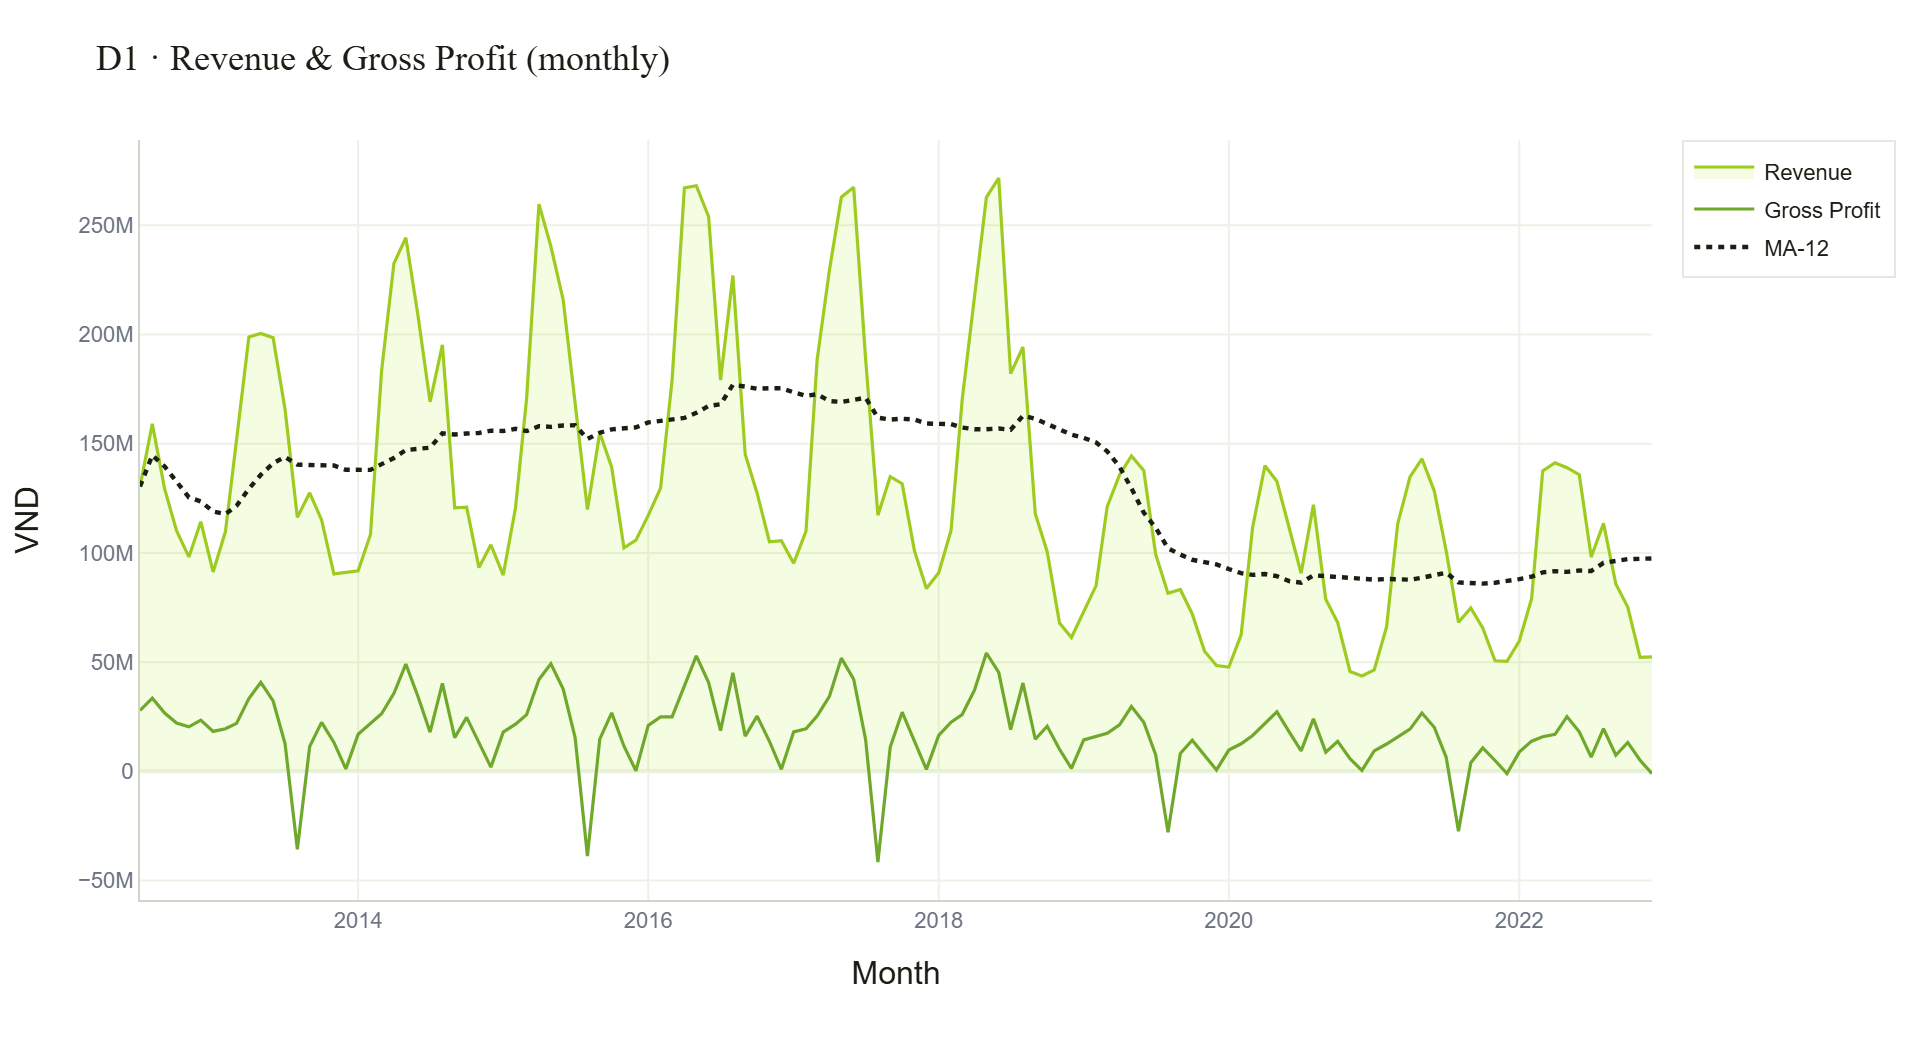
\includegraphics[width=\textwidth]{../../figures/D1/C1_revenue_trend.png}
        \caption{Doanh thu và lợi nhuận công ty theo ngày}
        \label{fig:rev_profit_year}
    \end{subfigure}
    \begin{subfigure}{0.5\textwidth}
        \centering
        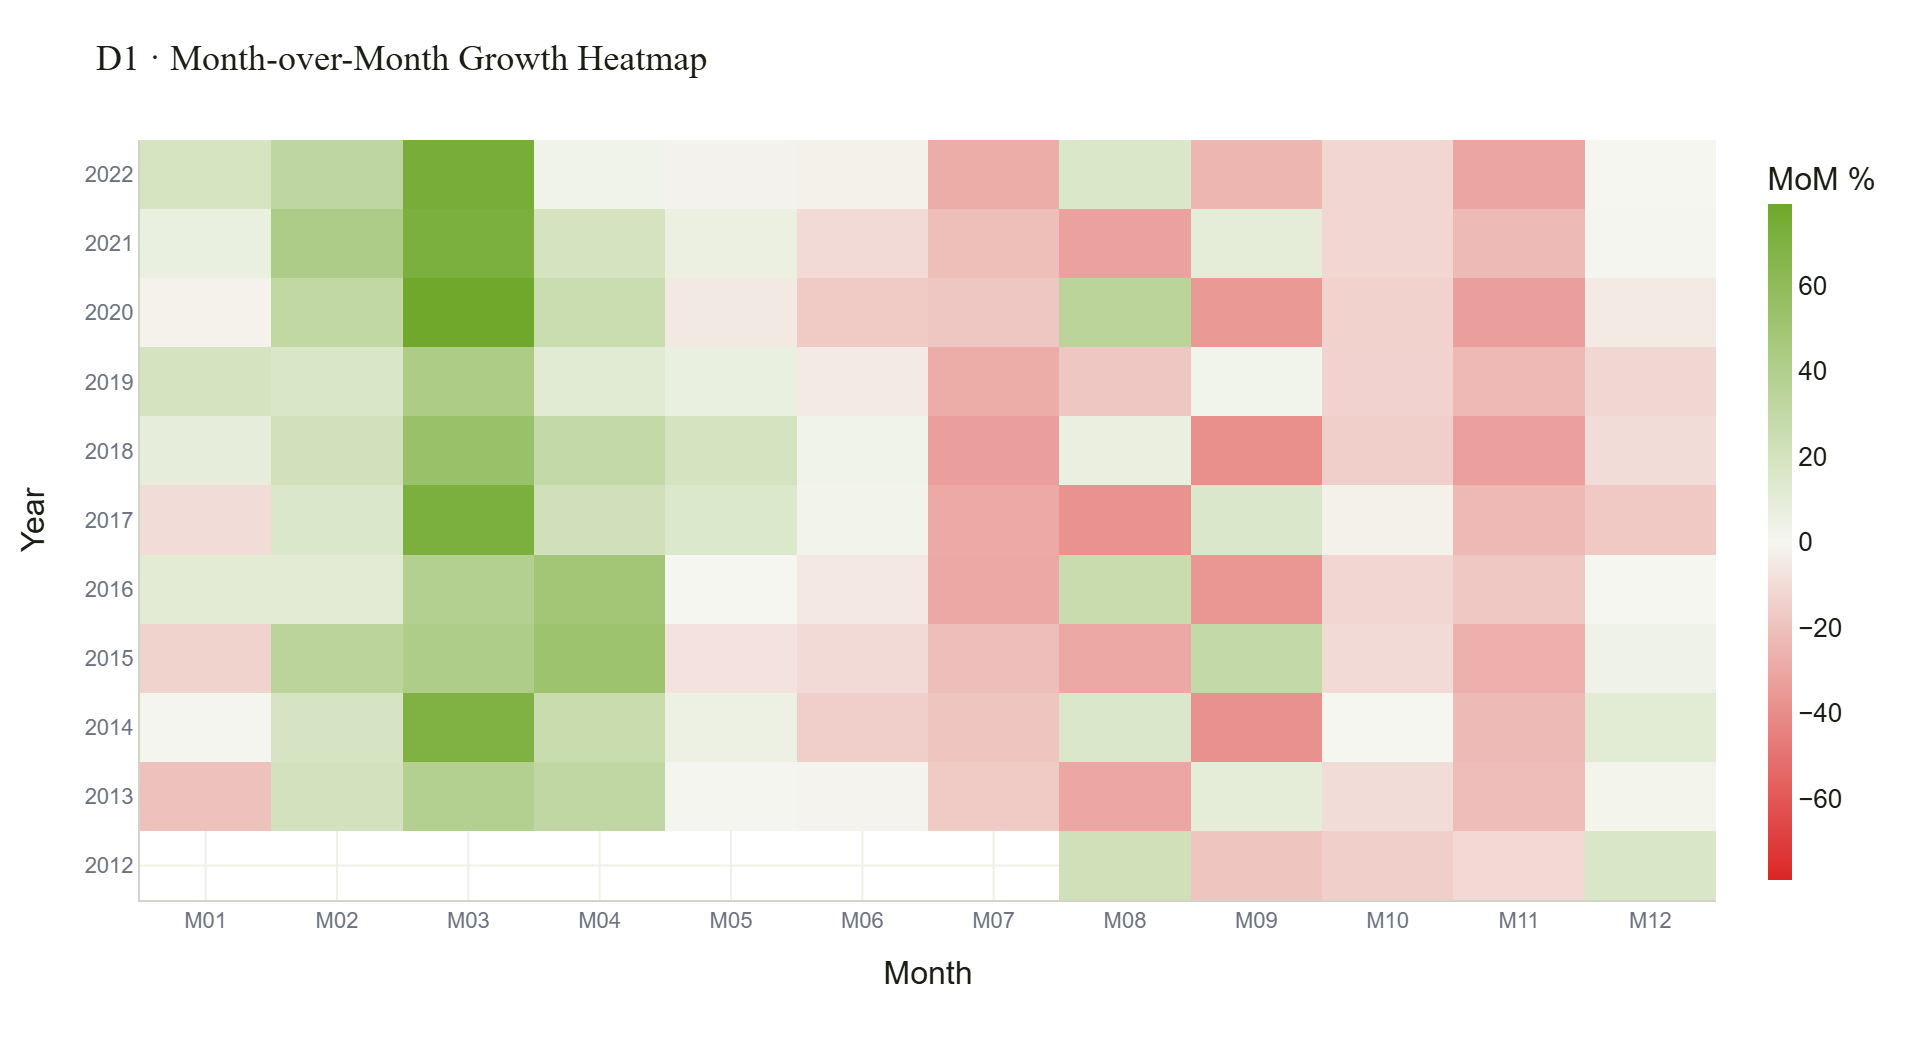
\includegraphics[width=\textwidth]{../../figures/D1/C2_mom_heatmap.png}
        \caption{Biểu đồ nhiệt thể hiện mức tăng trưởng theo từng tháng trong năm}
        \label{fig:growth}
    \end{subfigure}
    \caption{Biểu đồ thể hiện xu hướng thay đổi của doanh thu và lợi nhuận từ 2012-2022}
\end{figure}

\begin{figure}[h]
    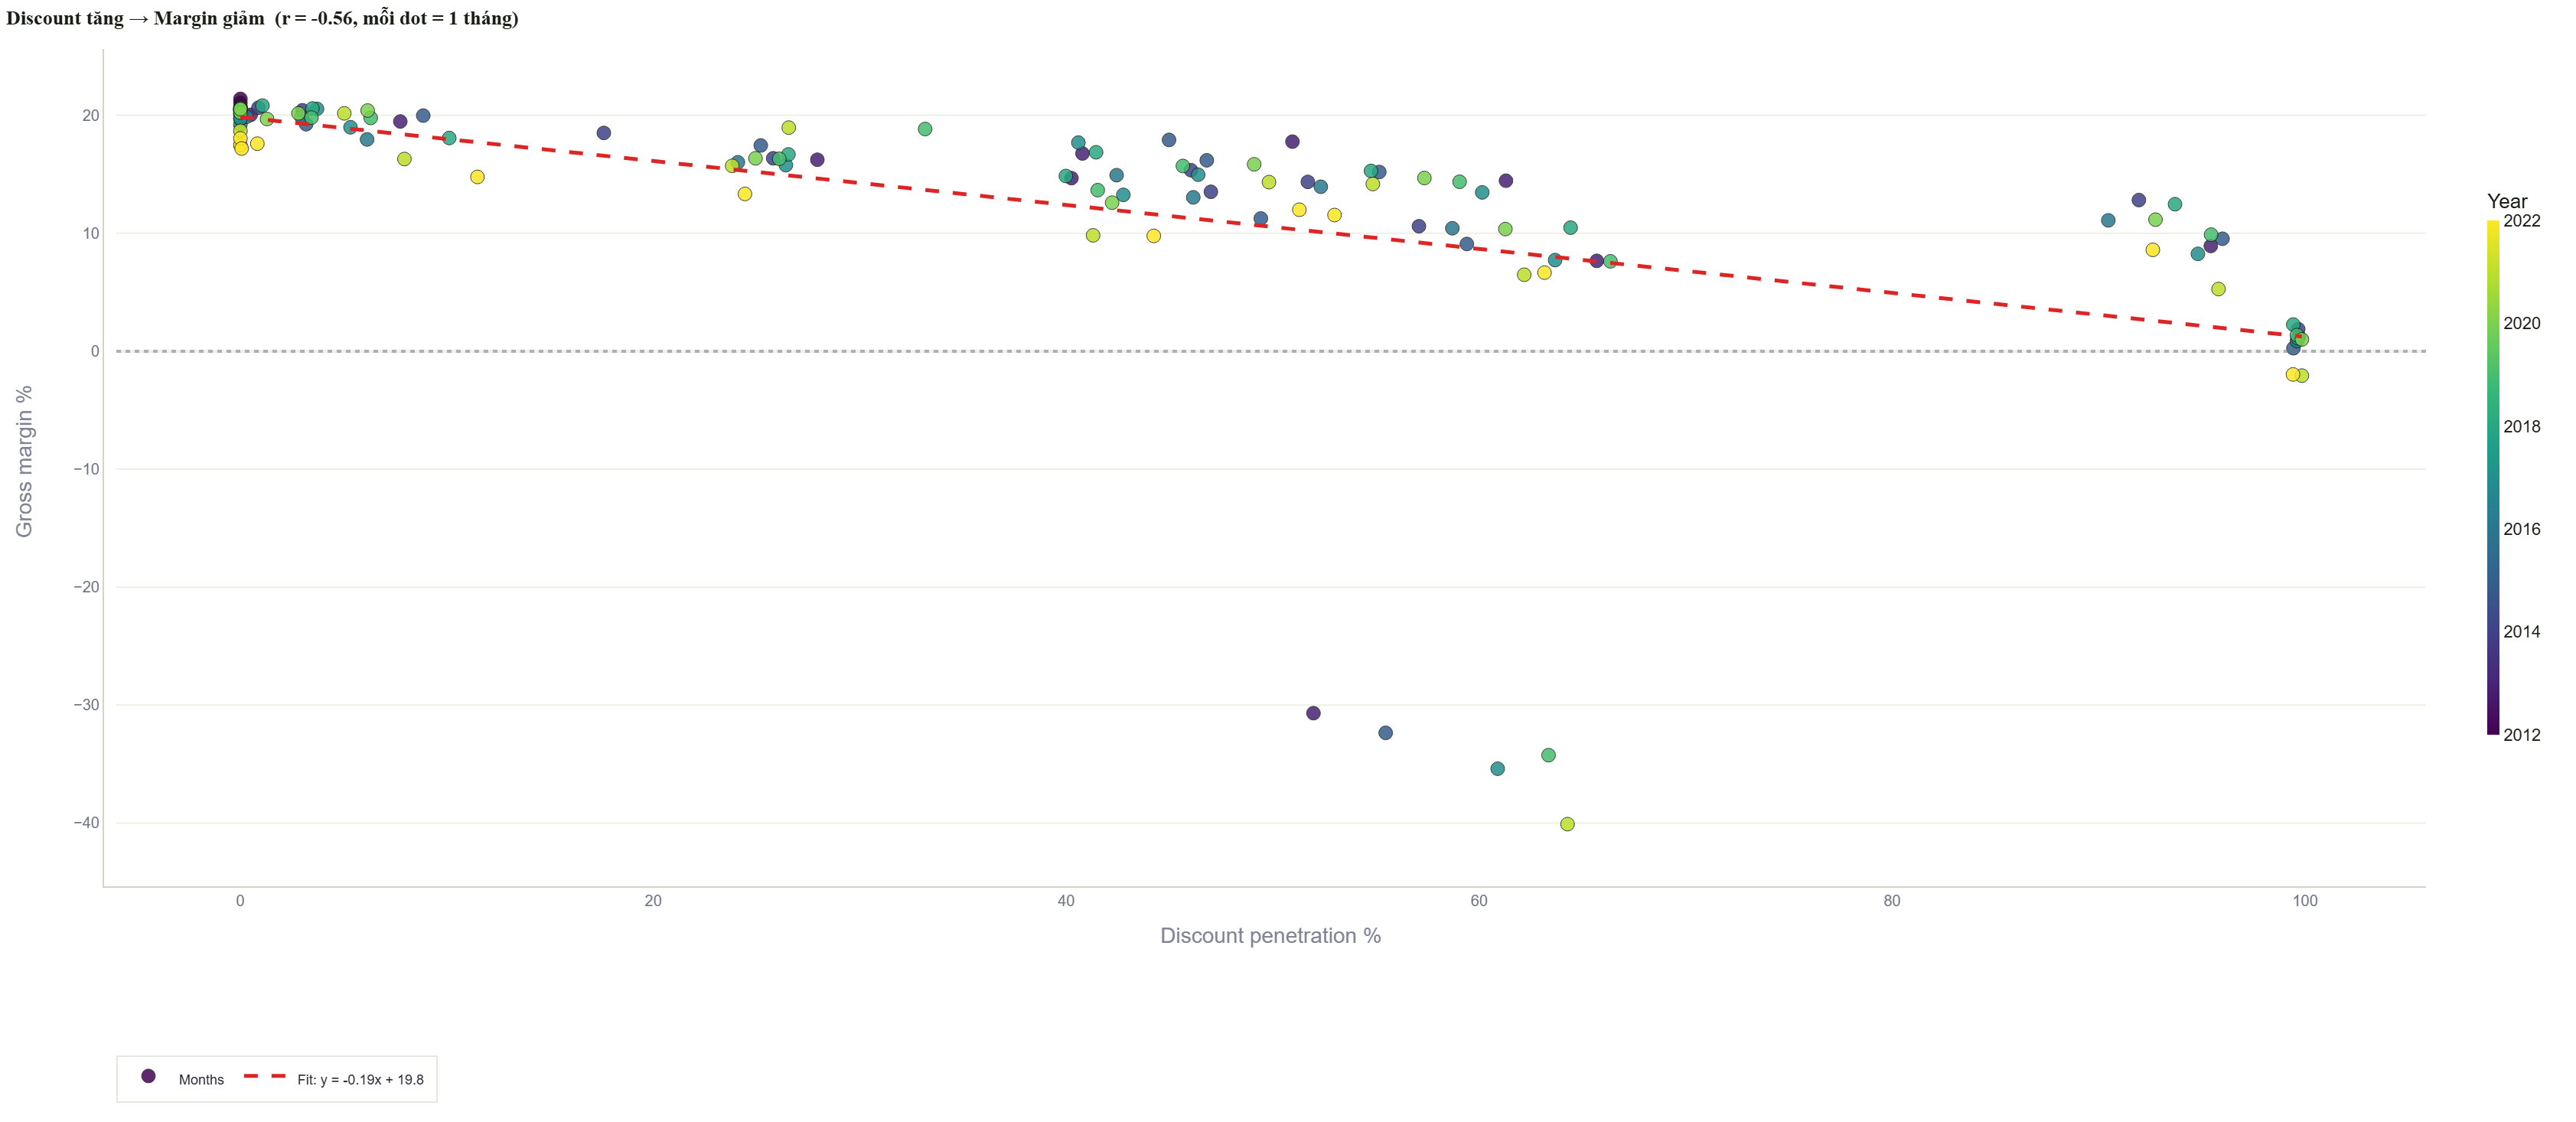
\includegraphics[width=\textwidth]{../../figures/D1/C1_discount_margin.png}
    \caption{Biểu đồ phân tán thể hiện mối quan hệ giữa biên lợi nhuận và mức discount được áp dụng}
    \label{fig:margin-discount}
\end{figure}

Ngược lại, doanh thu có xu hướng suy giảm bắt đầu từ tháng 7 về sau, với mức suy
giảm từ 10\%--20\%, với doanh thu trung bình theo nămh có dấu hiệu suy giảm từ
2018, thể hiện qua đường thẳng màu đen ở Biểu~đồ~\ref{fig:rev_profit_year}.

Xét về hiệu quả ở các mức giả sản phẩm trong những giai đoạn có chương trình
khuyến mãi, Biểu~đồ~\ref{fig:margin-discount}
cho thấy rằng mức tăng trưởng biên lợi nhuận thường có mối quan hệ nghịch biến
với mức ưu đãi được áp dụng.

% \vspace{-2\baselineskip}
\subsection{Phân khúc khách hàng và giá trị vòng đời}
% \subsubsection{Kênh tiếp cận chính}
%
% Cuối cùng, nhóm thực hiện đánh giá độ hiệu quả ở các kênh tiếp cận của công ty.
% Biểu~đồ~\ref{fig:acquisition-channel}
% cho thấy rằng công ty thu hút khách hàng thông qua ba kênh tiếp cận chính:
% \verb|paid_search|, \verb|social_media|, và \verb|organic_search|; trong đó,
% trung bình các khách trên những kênh này mang giá trị vòng đời trong khoảng
% 160,000 đồng.
%
% \begin{figure}[h]
%     \begin{center}
%         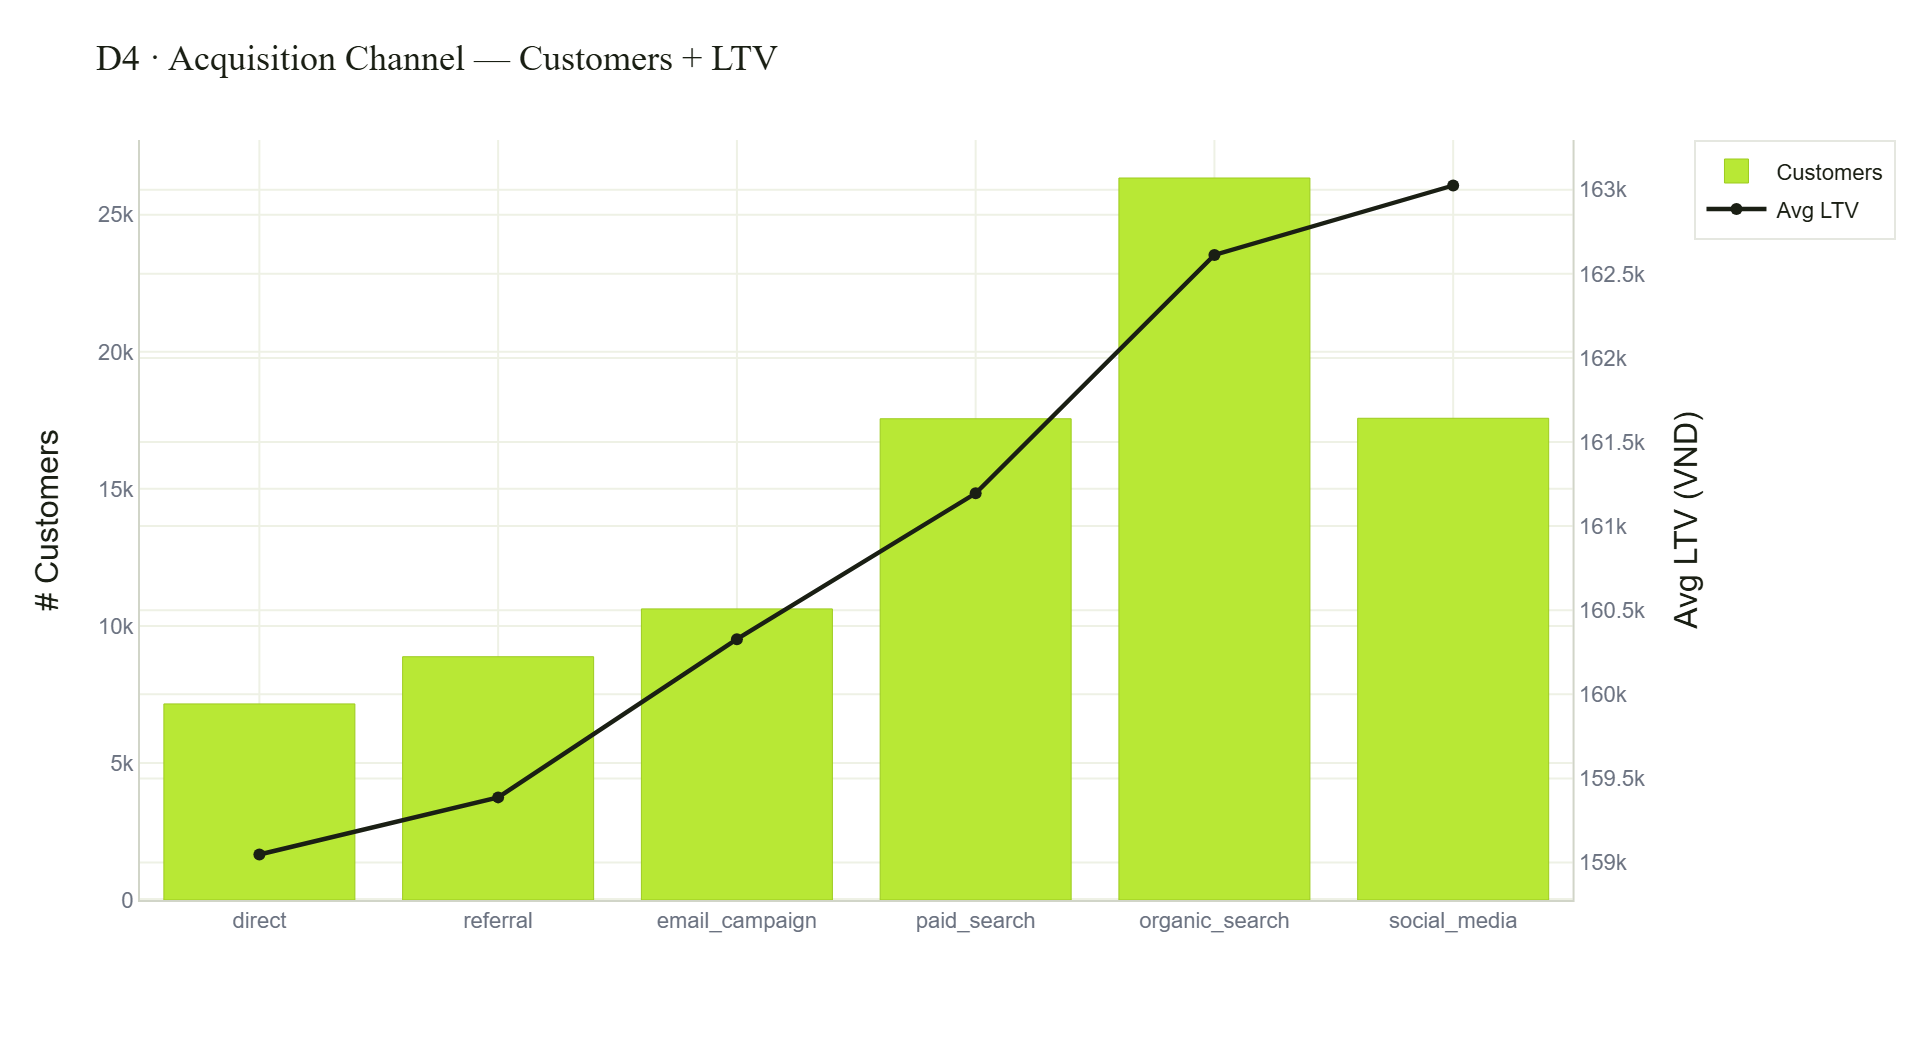
\includegraphics[width=0.7\textwidth]{../../figures/D4/C3_channel_ltv.png}
%     \end{center}
%     \caption{Biểu đồ cột thể hiện số lượng khách hàng được tiấp cận ở các kênh}
%     \label{fig:acquisition-channel}
% \end{figure}
% \vspace{-2\baselineskip}

\subsubsection{RFM Analysis}
Xét về hành vi mua hàng, biểu~đồ~\ref{fig:funnel}
cho thấy có đến 60\% khách hàng sẽ mua đến 3 đơn hàng, và gần 44\% khách hàng
sẽ mua từ 5 lần trở lần. Tuy nhiên, khi xét về khoảng cách giữa hai đơn hàng
liên tiếp, biểu~đồ~\ref{fig:cohort}
cho thấy tỉ lệ khách hàng sẽ đặt đơn kế tiếp trong cùng tháng thường chỉ nằm
trong mức 5--9\%; tức rằng, tần suất đặt hàng thường rất thấp xuyên xuốt các năm.

\begin{figure}[h]
    \begin{subfigure}{0.5\textwidth}
        \centering
        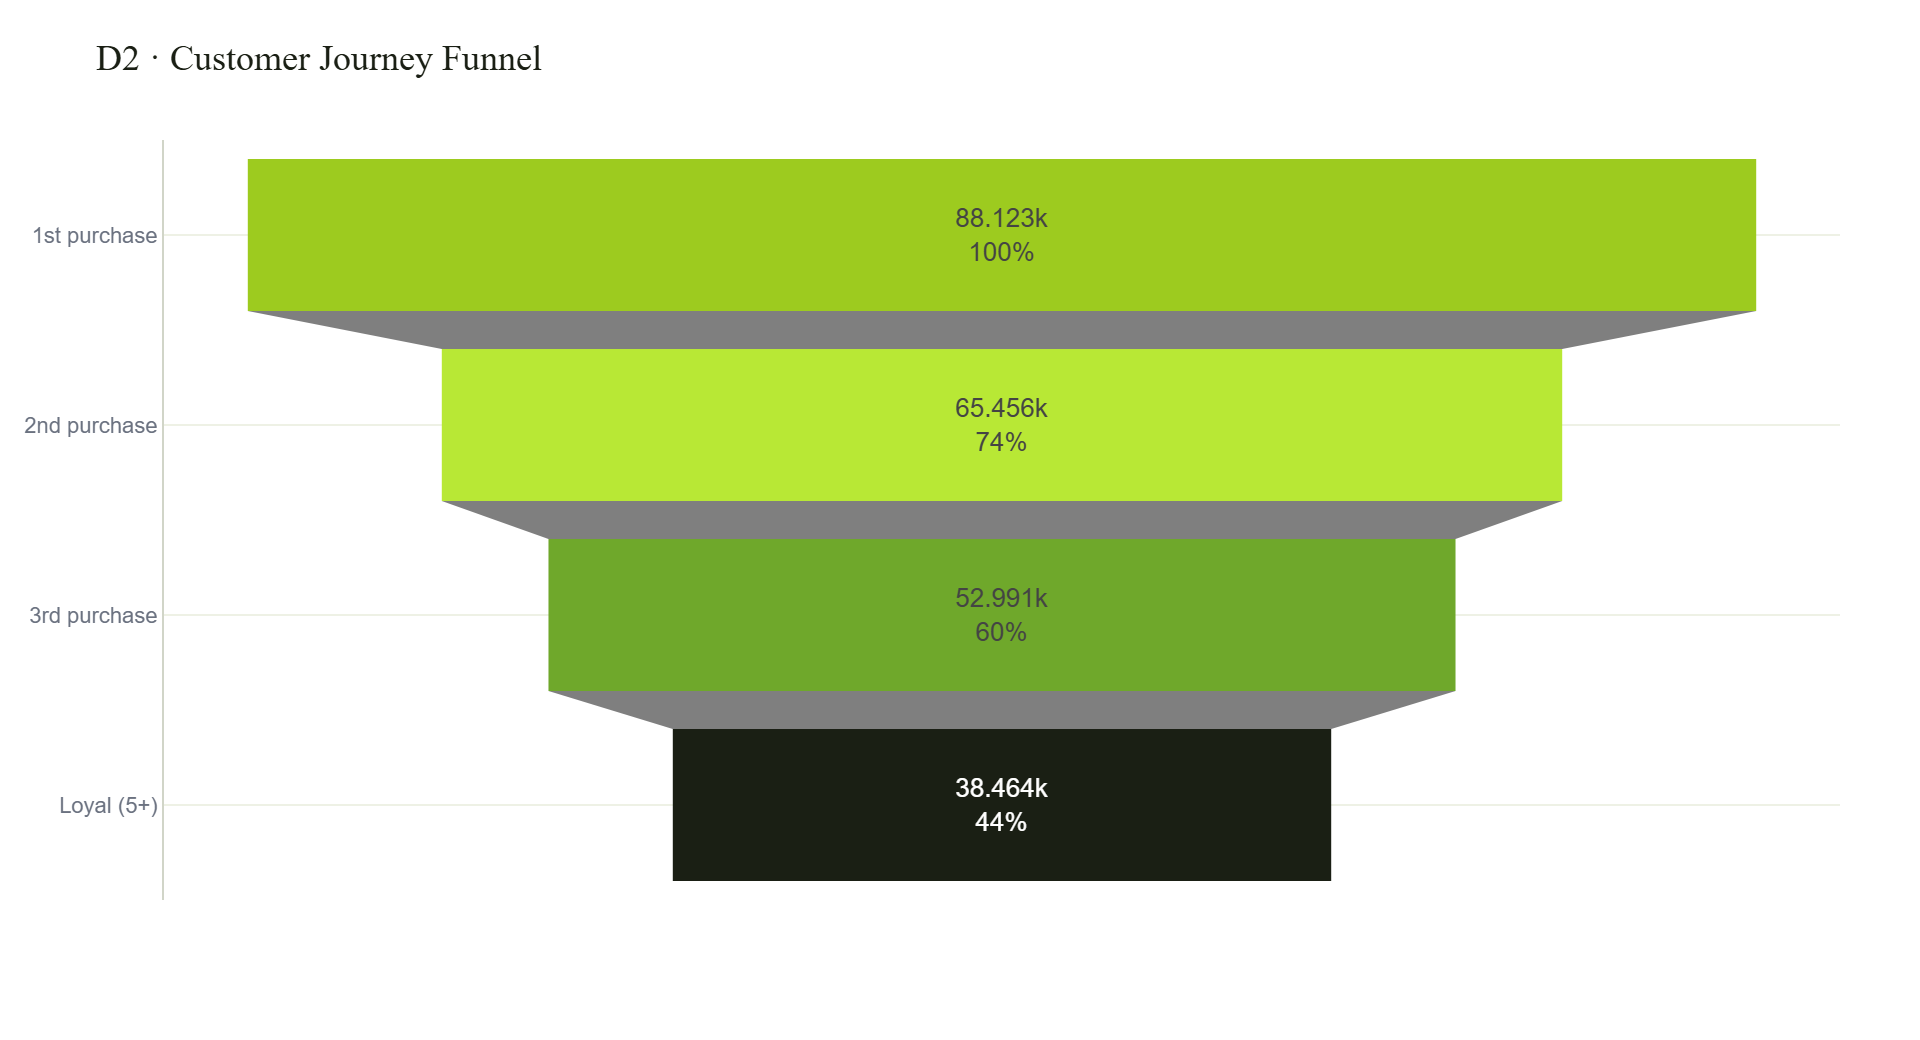
\includegraphics[width=0.95\textwidth]{../../figures/D2/C2_journey_funnel.png}
        \caption{Biểu đồ phễu thể hiện tỉ lệ mua lại của các khách hàng}
        \label{fig:funnel}
    \end{subfigure}
    \begin{subfigure}{0.5\textwidth}
        \centering
        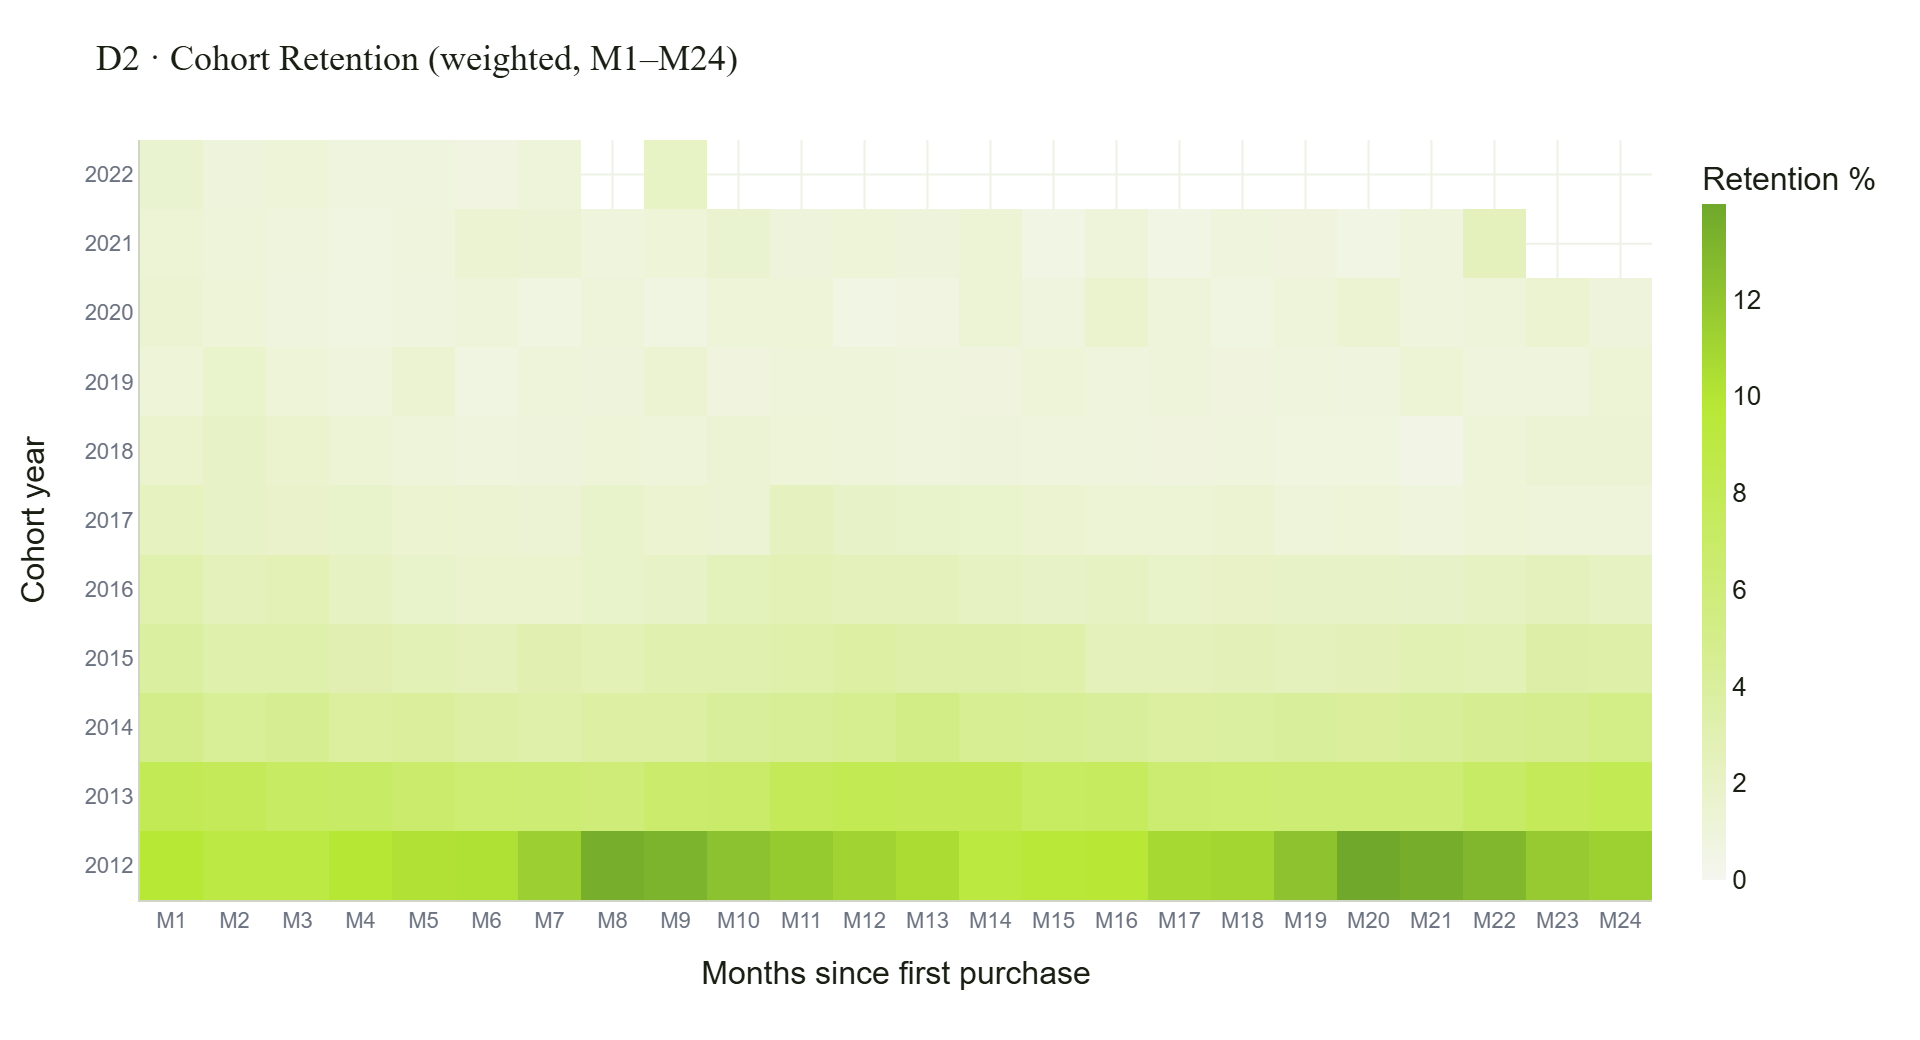
\includegraphics[width=0.95\textwidth]{../../figures/D2/C5_cohort_retention.png}
        \caption{Biểu đồ nhiệt thể hiện tỉ lệ đặt đơn tiếp theo trong cùng tháng
            của các khách hàng}
        \label{fig:cohort}
    \end{subfigure}
    \caption{Các biểu đồ thể hiện hành vi mua lại của các khách hàng}
\end{figure}

\vspace{-0.5\baselineskip}
Nhóm thực hiện phân tích Recency-Frequency-Monetary (RFM) nhằm đánh giá giá trị
vòng đời khách hàng công ty, tại thời điểm 01/01/2023. Để thực hiện phân nhóm
khách hàng, nhóm sử dụng thang đo được thể hiện qua Bảng~\ref{tab:rfm-groups}.

\begin{table}[h]
  \caption{Customer Segmentation based on RFM Scores}
  \label{tab:rfm-groups}
  \centering
  \begin{tabular}{lccc}
    \toprule
    \multicolumn{4}{c}{RFM Segments} \\
    \cmidrule(r){1-4}
    Segment & Recency (R) & Frequency (F) & Monetary (M) \\
    \midrule
    Champions            & 4--5 & 4--5 & any \\
    Loyal Customers      & 3--5 & 3--5 & any \\
    Cant Lose Them       & 1--2 & 4--5 & $\geq 4$ \\
    Potential Loyalists  & 3    & 1--2 & $\geq 3$ \\
    New Customers        & 4--5 & 1--2 & any \\
    About To Sleep       & 3    & 1--2 & $< 3$ \\
    At Risk              & 1--2 & 3--5 & any \\
    Lost                 & 1--2 & 1--2 & any \\
    \bottomrule
  \end{tabular}
\end{table}

Biểu~đồ~\ref{fig:customer-rf-group}
cho thấy công ty có số lượng lớn khách hàng thuộc ba nhóm Lost, Champions, và
Loyal Customers. Chi tiết này có thể được giải thích bởi thời gian hoạt động
kinh doanh khá lâu, dẫn đến sự tích lũy ở số lượng các khách hàng thân quen, cũng
như khách hàng không chuyển đổi thành công.

\begin{figure}[h]
    \centering
    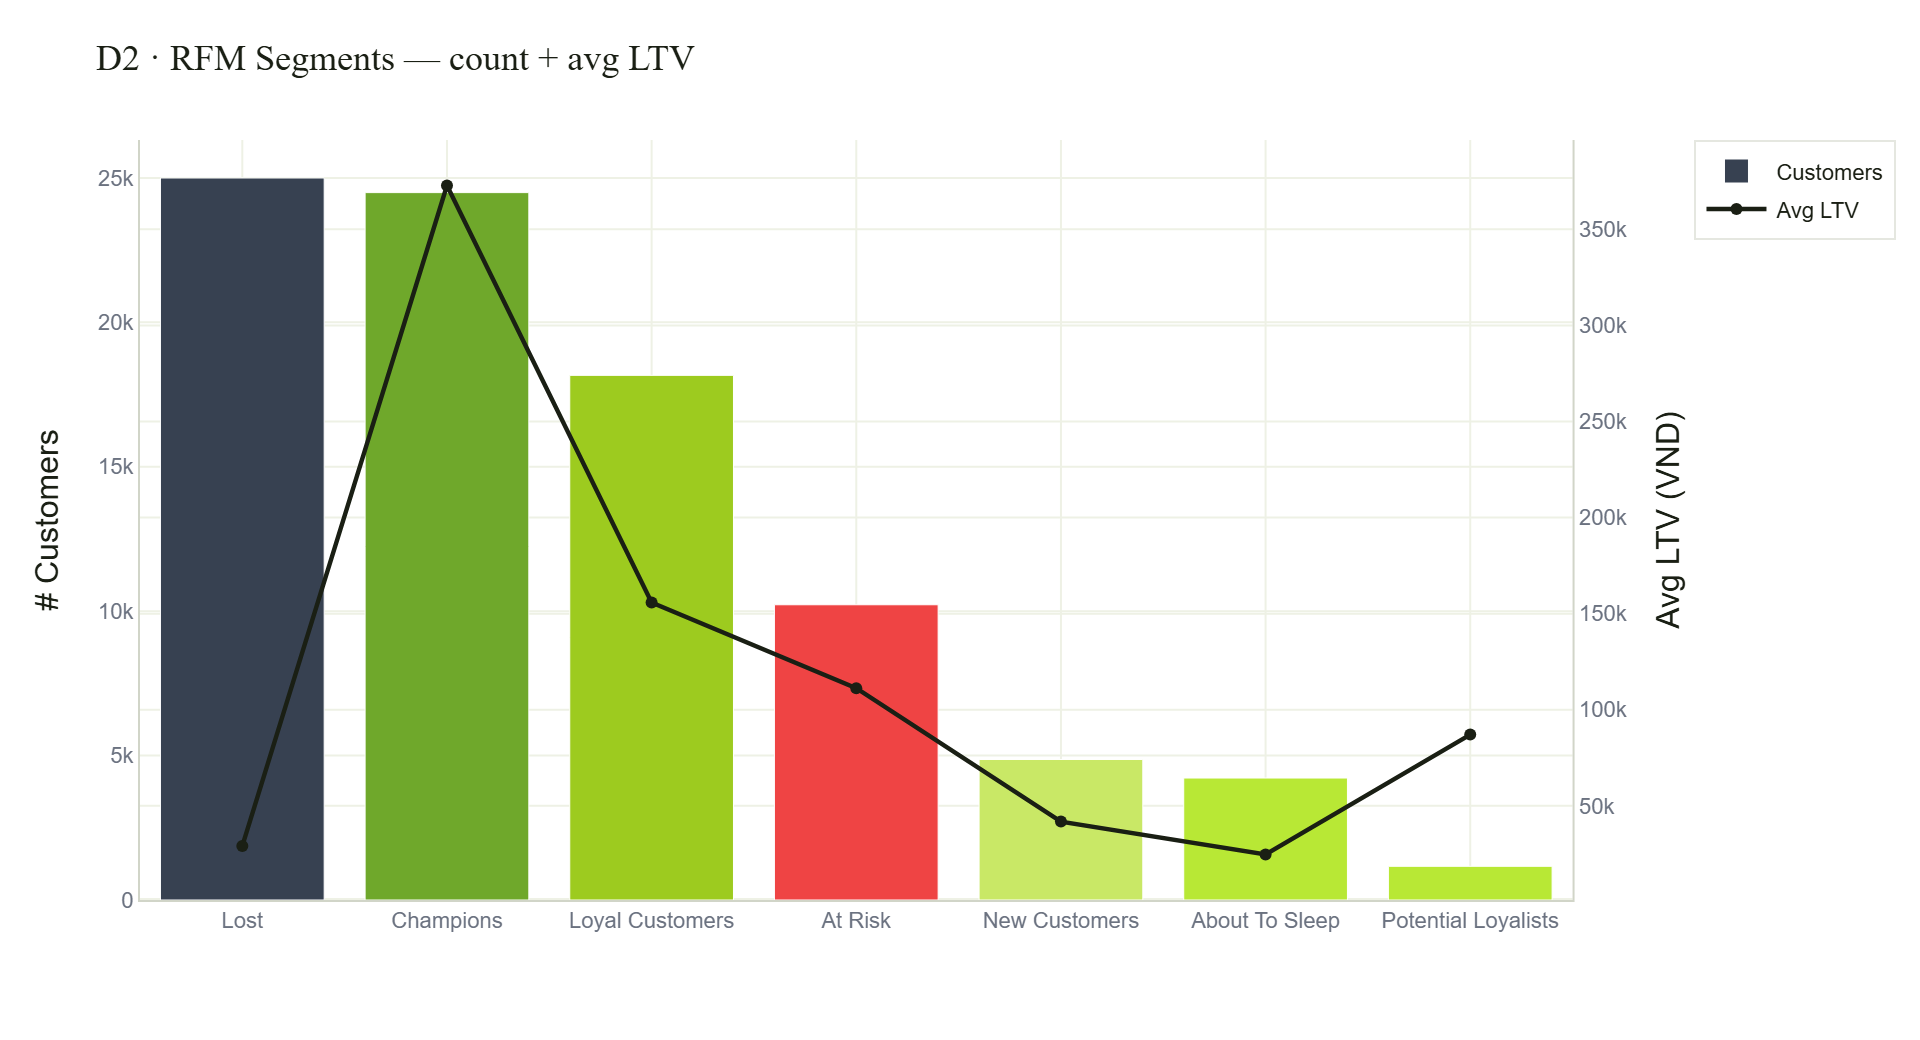
\includegraphics[width=.7\textwidth]{../../figures/D2/C1_rfm_segments.png}
    \caption{Biểu đồ cột thể hiện giá trị vòng đời khách hàng theo nhóm}
    \label{fig:customer-rf-group}
\end{figure}

Ngược lại, số lượng khách hàng thuộc nhóm New Customers và Potential Loyalists
chỉ chiếm khoảng 6.8\% tổng số khách hàng, cho thấy công ty chưa có cách tiếp cận
hiệu quả nhằm tích lũy các nhóm khách hàng mới.

\begin{figure}[h]
    \centering
    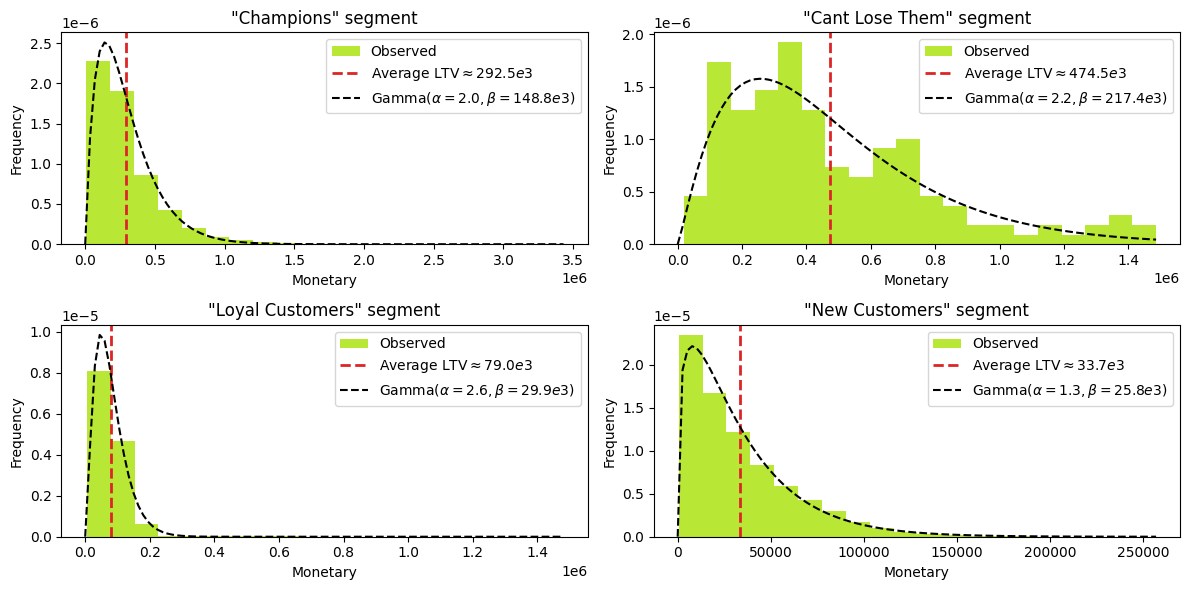
\includegraphics[width=.7\textwidth]{../../figures/D2/monetary-distribution-segment.png}
    \caption{Phân phối giá trị monetary ở bốn nhóm Champions, Cant Lose Them,
        Loayal Customers, và New Customers. Giá trị $\alpha$ đại diện cho số
        đơn trung bình khách hàng đặt, tính tới thời điểm 01/01/2023. Giá
        trị $\beta$ đại diện cho tổng giá trị trên mỗi đơn khách hàng đặt.}
    \label{fig:monetary-dist}
\end{figure}

\vspace{-.5\baselineskip}
Đồng thời, nhằm có ước lượng tổng thể hơn về tổng giá trị vòng đời của một khách
hàng đặc trưng trong các phân khúc, nhóm đã thực hiện tính MLE và fit các giá
trị monetary theo phân phối Gamma, thể hiện ở Biểu~đồ~\ref{fig:monetary-dist}.
Các ước lượng phân phối cho thấy giá trị vòng đời trung bình tương ứng với
Biểu~đồ~\ref{fig:customer-rf-group}.

Đặc biệt, nhóm Loyal Customers có sự khác biệt đáng kể về giá trị đơn hàng, với
hầu hết giá trị đơn hàng tập trung trong khoảng dưới 200,000 đồng. Trong khi đó,
nhóm Champions có đuôi phân phối lệch phải nhiều hơn về các trị giá đơn hàng từ
500,000 đồng trở lên.

Theo đó, nhóm thấy rằng việc tập trung quá mức vào các nhóm khách hàng trung
thành mang nhiều rủi rỏ về các chi phí công ty cần bỏ ra để duy trì sự hài lòng
khách hàng. Do đó, công ty cần có thêm các chiến lược thu hút khách hàng mới,
nhằm tăng cơ hội chuyển đổi và tích lũy khách hàng trung thành.

\subsection{Hiệu quả kinh doanh các sản phẩm}

Nhóm phát hiện rằng một trong những nhóm hàng phổ biến nhất của công ty là nhóm
Streetwear, với doanh thu chiếm gần 80\% tổng doanh thu trên các mặt hàng, thể
hiện ở biểu~đồ~\ref{fig:product-cate}.

% Dựa trên mức lợi nhuận biên 20\%, việc cắt giảm chi phí của nhóm hàng này nhằm
% tăng mức biên là một chiến lược tiềm năng nhằm đẩy mạnh mức tăng trưởng lợi nhuận
% của doanh nghiệp.

Theo đó, nhóm đề xuất doanh nghiệp cắt giảm chi phí hoặc loại bỏ các dòng sản phẩm
kinh doanh chưa hiệu quả như Casual và GenZ. Đồng thời, doanh nghiệp có thể tối
ưu hóa dây chuyền sản xuất ở nhóm hàng Streetwear với mục tiêu tối đa hóa biên
lợi nhuận sản phẩm, tạo cơ hội khai thác giá trị tiềm năng.

\begin{figure}[h]
    \begin{subfigure}{0.5\textwidth}
        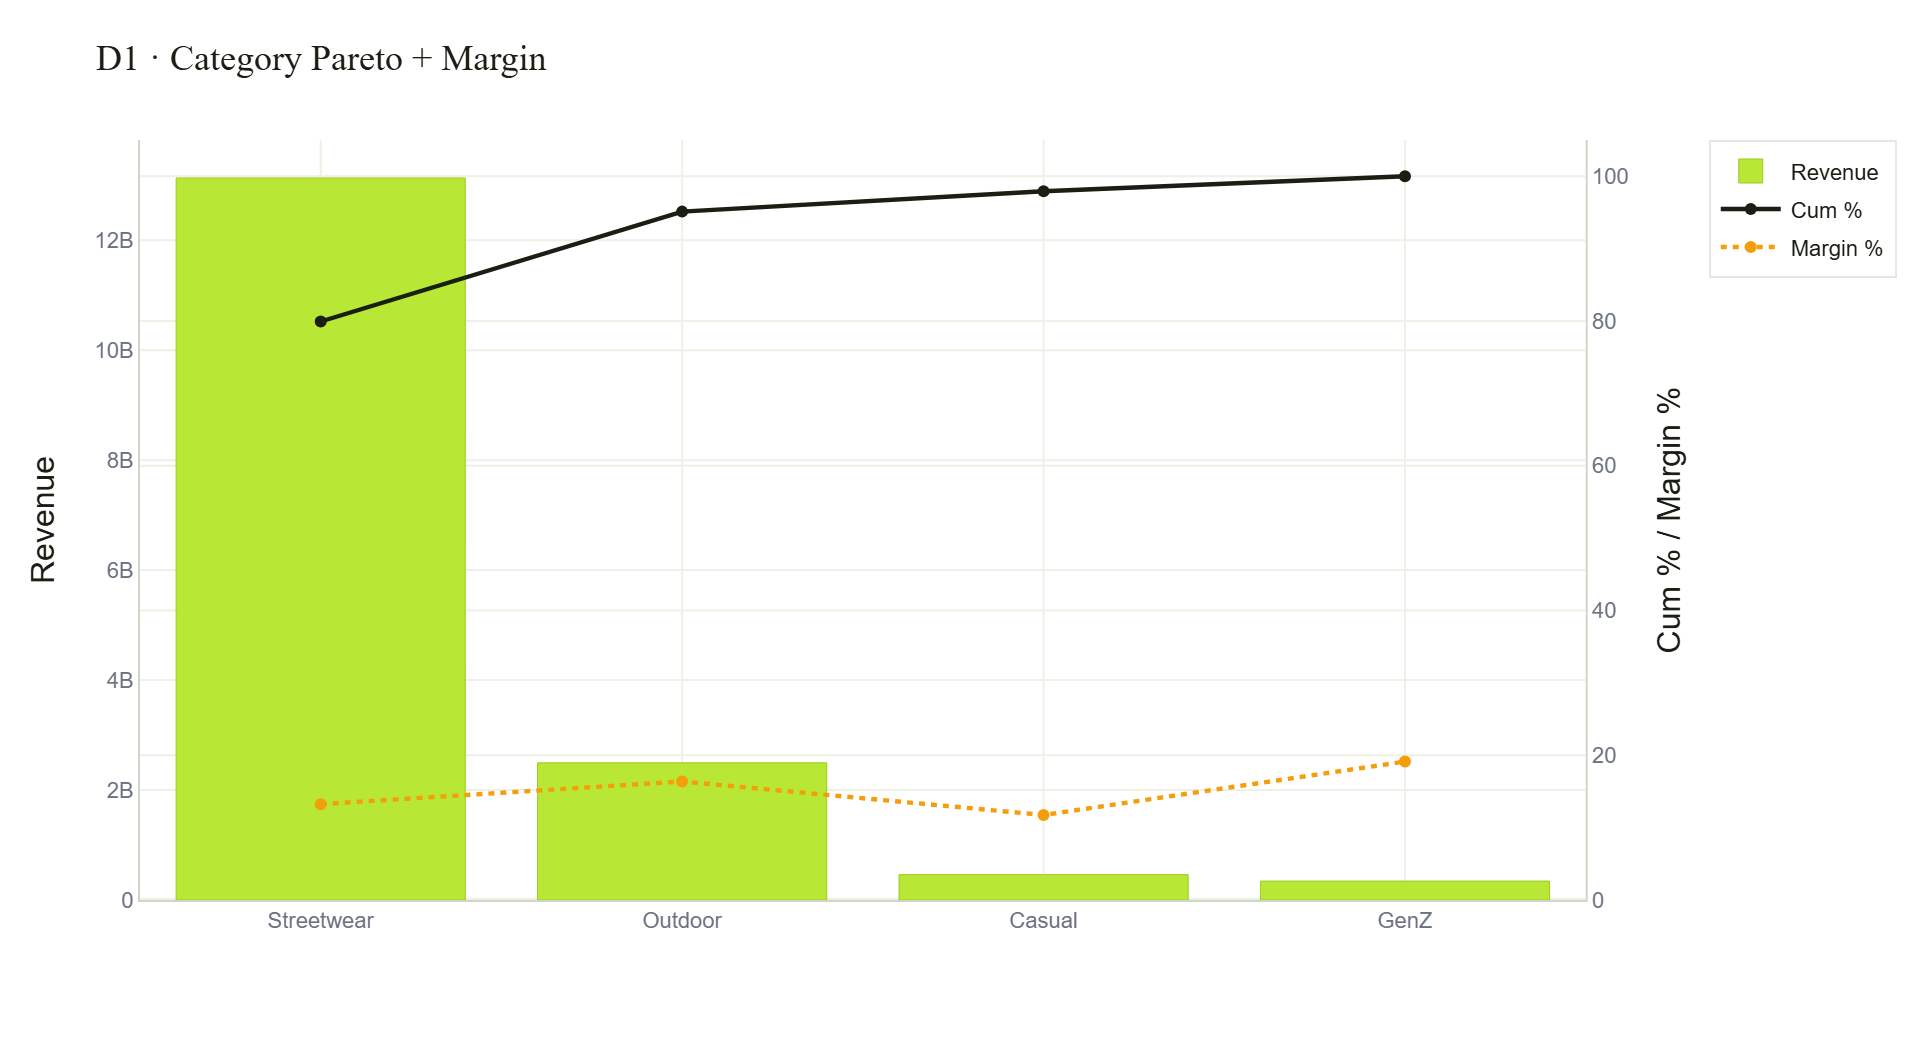
\includegraphics[width=\textwidth]{../../figures/D1/C4_category_pareto.png}
        \caption{Biểu đồ cột thể hiện doanh thu của bốn nhóm sản phẩm chính}
        \label{fig:product-cate}
    \end{subfigure}
    \begin{subfigure}{0.5\textwidth}
        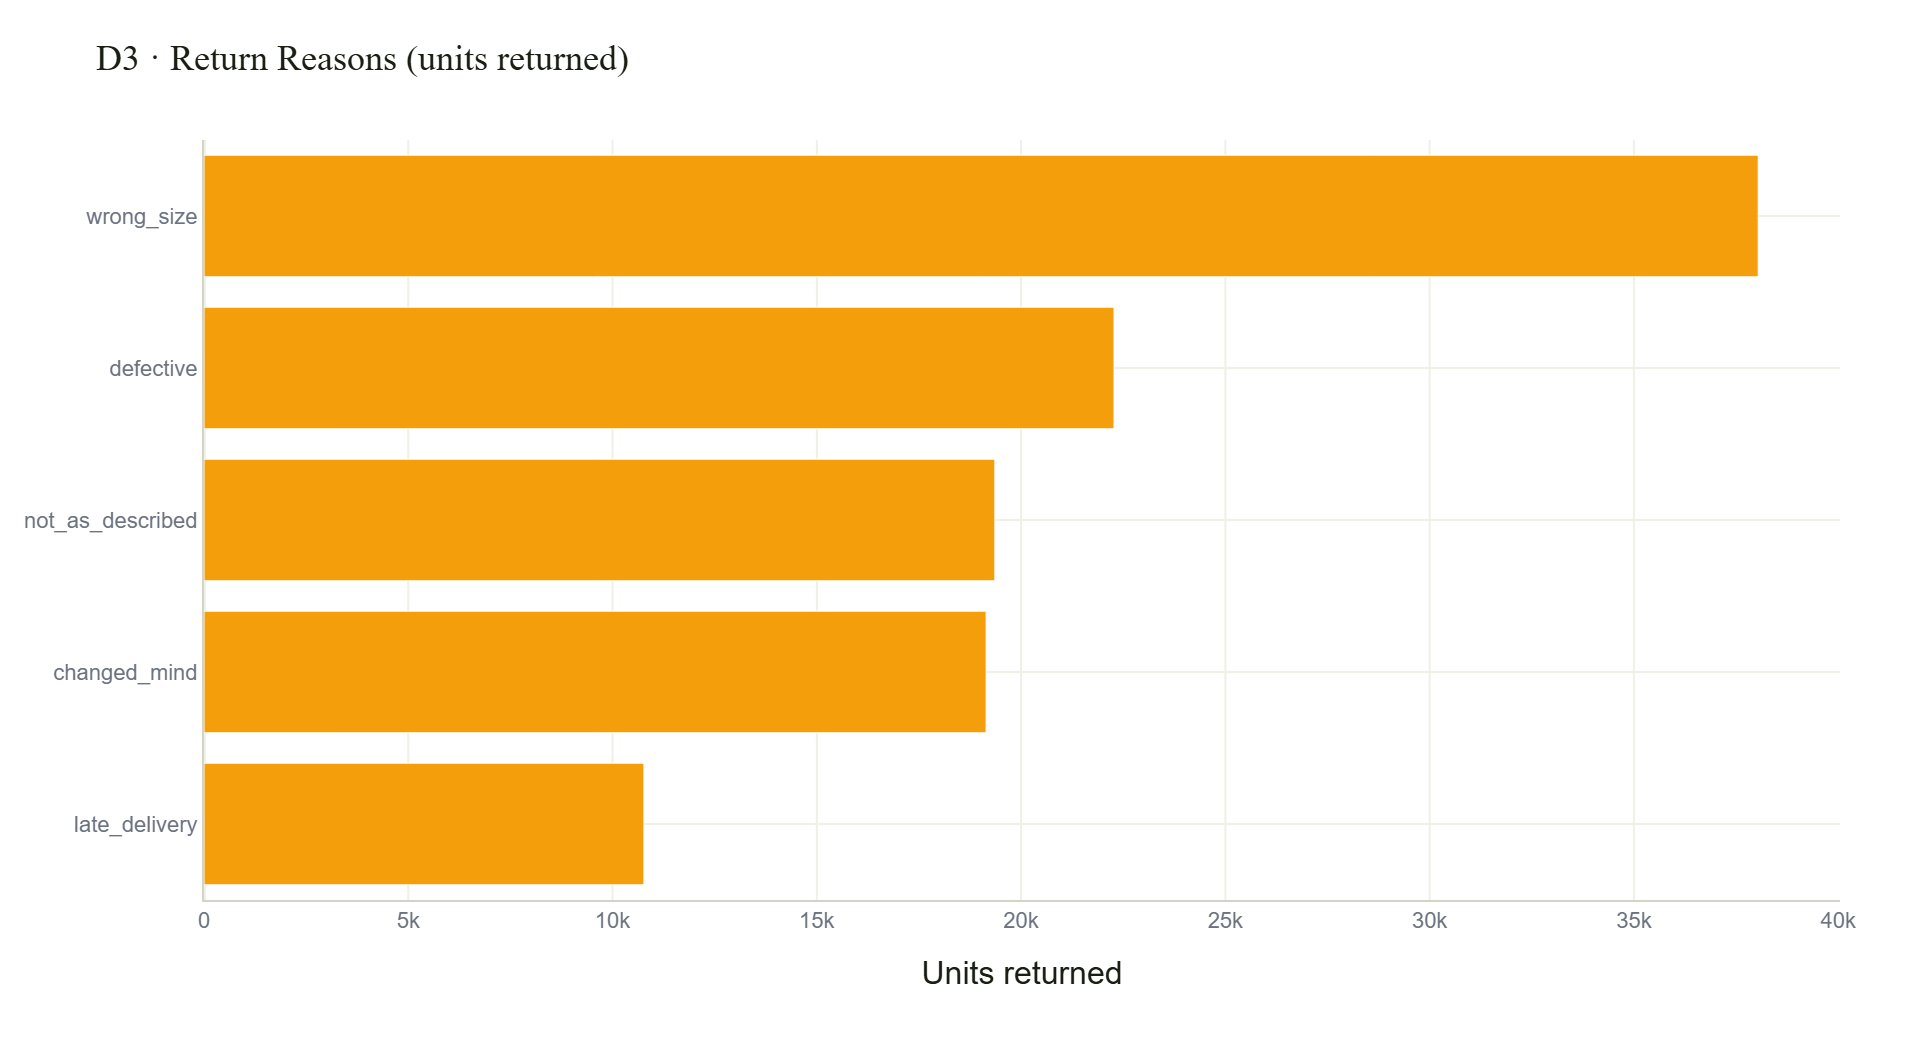
\includegraphics[width=\textwidth]{../../figures/D3/C2_return_reasons.png}
        \caption{Biểu đồ cột thể hiện số lượng các lý do trả hàng}
        \label{fig:returns}
    \end{subfigure}
    \caption{Các thống kê theo nhóm hàng và mặt hàng}
\end{figure}

\vspace{-.5\baselineskip}
Cuối cùng, nhóm nhấn mạnh chi tiết các mặt hàng được trả lại thường đến từ việc
giao sản phẩm không đúng kích cỡ, dựa vào Biểu~đồ~\ref{fig:returns}.
Theo đó, công ty cần xây dựng quy trình đóng đơn nghiêm ngặt nhằm tránh tình
trạng giao sai sản phẩm, giảm ảnh hưởng đến trải nghiệm khách hàng, và tăng biên
lọi nhuận doanh nghiệp.

\subsection{Tổng quan phân tích}

\section{Xây dựng mô hình dự báo doanh thu}
\subsection{Data và Model Pipeline}
\subsection{Kết quả huấn luyện mô hình}

\end{document}
